\documentclass[10pt]{article}

% Packages
\usepackage[margin=1.5in]{geometry}  % Wider margins like Attention paper
\usepackage{times}                   % Times font
\usepackage{graphicx}
\usepackage{hyperref}
\usepackage{amsmath}
\usepackage{amssymb}
\usepackage{booktabs}
\usepackage{multirow}
\usepackage{array}

% Remove page numbers for arXiv style
\pagestyle{plain}

% Hyperref setup
\hypersetup{
    colorlinks=true,
    linkcolor=black,
    urlcolor=black,
    citecolor=black
}

% Custom title formatting to match Attention paper
\makeatletter
\def\@maketitle{%
  \newpage
  \null
  \vskip 2em%
  \begin{center}%
    \rule{\textwidth}{1pt}%
    \vskip 1em%
    {\LARGE \bfseries \@title \par}%
    \vskip 1em%
    \rule{\textwidth}{1pt}%
    \vskip 2em%
    {\large
      \lineskip .5em%
      \begin{tabular}[t]{c}%
        \@author
      \end{tabular}\par}%
    \vskip 1em%
  \end{center}%
  \par
  \vskip 1.5em}
\makeatother

\title{SeizureTransformer on TUSZ: A 27-137x Performance Gap Between\\Claims and Reproducible Evaluation}

\author{
  \textbf{John H. Jung, MD, MS}\\
  Independent Researcher\\
  \texttt{JJ@novamindnyc.com}
}

\date{}  % No date

\begin{document}

\maketitle

\begin{center}
\textbf{Abstract}
\end{center}

SeizureTransformer reports $\sim$1 false alarm per 24 hours on the EpilepsyBench Dianalund dataset. Despite being trained on the Temple University Hospital Seizure (TUSZ) dataset, it has not been evaluated on TUSZ using Temple's official scoring software. We provide, to our knowledge, the first such evaluation with NEDC v6.0.0 and find a 27--137$\times$ gap between benchmark claims and clinical reality.

We evaluate the authors' pretrained model on TUSZ v2.0.3's held-out set (865 files, 127.7 hours) and assess identical predictions with four scoring methodologies. With NEDC OVERLAP, the model produces 26.89 FA/24h; with SzCORE, 8.59 FA/24h ($\approx$3.1$\times$ lower due solely to scoring tolerances); with NEDC TAES, 136.73 FA/24h.

When tuned toward deployment goals, the model cannot meet clinical thresholds with NEDC scoring: targeting 10 FA/24h achieves only 33.90\% sensitivity, far below the 75\% sensitivity goal for clinical systems (Roy et al., 2021). Acceptable false-alarm rates occur only under SzCORE's permissive tolerances.

We contribute a reproducible NEDC evaluation pipeline, operating points tailored to clinical targets, and quantitative evidence that scoring choice alone drives multi-fold differences. Dataset-matched, clinician-aligned evaluation is essential for credible seizure-detection claims.

\section{Introduction}

Epilepsy affects 50 million people worldwide, with approximately 30\% experiencing drug-resistant seizures that require continuous EEG monitoring for optimal management. The promise of automated seizure detection has tantalized the field for decades, with recent deep learning advances suggesting we may finally be approaching clinical viability. SeizureTransformer, winner of the 2025 EpilepsyBench Challenge, achieved remarkable performance with just 1 false alarm per 24 hours on the Dianalund dataset—a result that would meet stringent clinical deployment standards. Yet when we evaluated this same model on the dataset it was trained on, using the official scoring software designed for that dataset, we discovered false alarm rates 27 to 137 times higher than claimed, depending on the scoring methodology employed.

SeizureTransformer represents a significant architectural advance in seizure detection, combining U-Net's proven biomedical segmentation capabilities with Transformer self-attention mechanisms to capture both local and global EEG patterns. The model was trained on a subset of the Temple University Hospital Seizure (TUSZ) dataset (v1.5.2; $\sim$910 hours) together with the Siena Scalp EEG Database ($\sim$128 hours). TUSZ itself is the largest publicly available seizure corpus, but the model's training used a subset as reported by the authors. Its victory in EpilepsyBench 2025, achieving 37\% sensitivity at 1 FA/24h on the Dianalund dataset, established it as the state-of-the-art in automated seizure detection. The authors openly shared their pretrained weights, enabling reproducible research and clinical validation.

Despite this success, a critical evaluation gap exists. While SeizureTransformer was trained on TUSZ's training set, no published evaluation exists using TUSZ's carefully designed, patient-disjoint held-out evaluation set. This 127.7-hour test set, containing 865 files from 43 patients with 469 seizures, was specifically created to enable valid performance assessment. Moreover, Temple University developed the NEDC (Neural Event Detection Competition) scoring software explicitly to match TUSZ's annotation philosophy, ensuring consistent evaluation standards. The absence of TUSZ evaluation is not unique to SeizureTransformer—it reflects a broader pattern where models trained on datasets are evaluated elsewhere, with results reported using varying scoring methodologies.

The choice of scoring methodology profoundly impacts reported performance. The seizure detection community employs multiple evaluation standards, each serving different purposes. NEDC implements strict temporal precision matching Temple's conservative annotation guidelines. In contrast, SzCORE—the EpilepsyBench standard—adds 30-second pre-ictal and 60-second post-ictal tolerances around ground truth events, designed to reward clinically useful early warnings. These philosophical differences are not matters of right or wrong but reflect different priorities: research precision versus clinical utility. However, when the same predictions can yield anywhere from 8.59 to 136.73 false alarms per 24 hours purely based on scoring choice, the lack of standardized reporting becomes problematic.

We present, to our knowledge, the first evaluation of SeizureTransformer on TUSZ's held-out test set using Temple's NEDC v6.0.0 scoring software. Our systematic comparison evaluates identical model predictions using four scoring methodologies: NEDC TAES (time-aligned event scoring), NEDC OVERLAP (binary any-overlap), our Python implementation of OVERLAP (achieving perfect parity with NEDC), and SzCORE. At the paper's default parameters ($\theta$=0.8, kernel=5, duration=2.0s), we observe 45.63\% sensitivity at 26.89 FA/24h with NEDC OVERLAP—a 27-fold increase from the Dianalund benchmark claim. The same predictions yield 136.73 FA/24h with NEDC TAES (137-fold increase) and 8.59 FA/24h with SzCORE. This 3.1-fold difference between NEDC OVERLAP and SzCORE stems entirely from scoring methodology, independent of model architecture or parameters.

\begin{figure}[h]
\centering
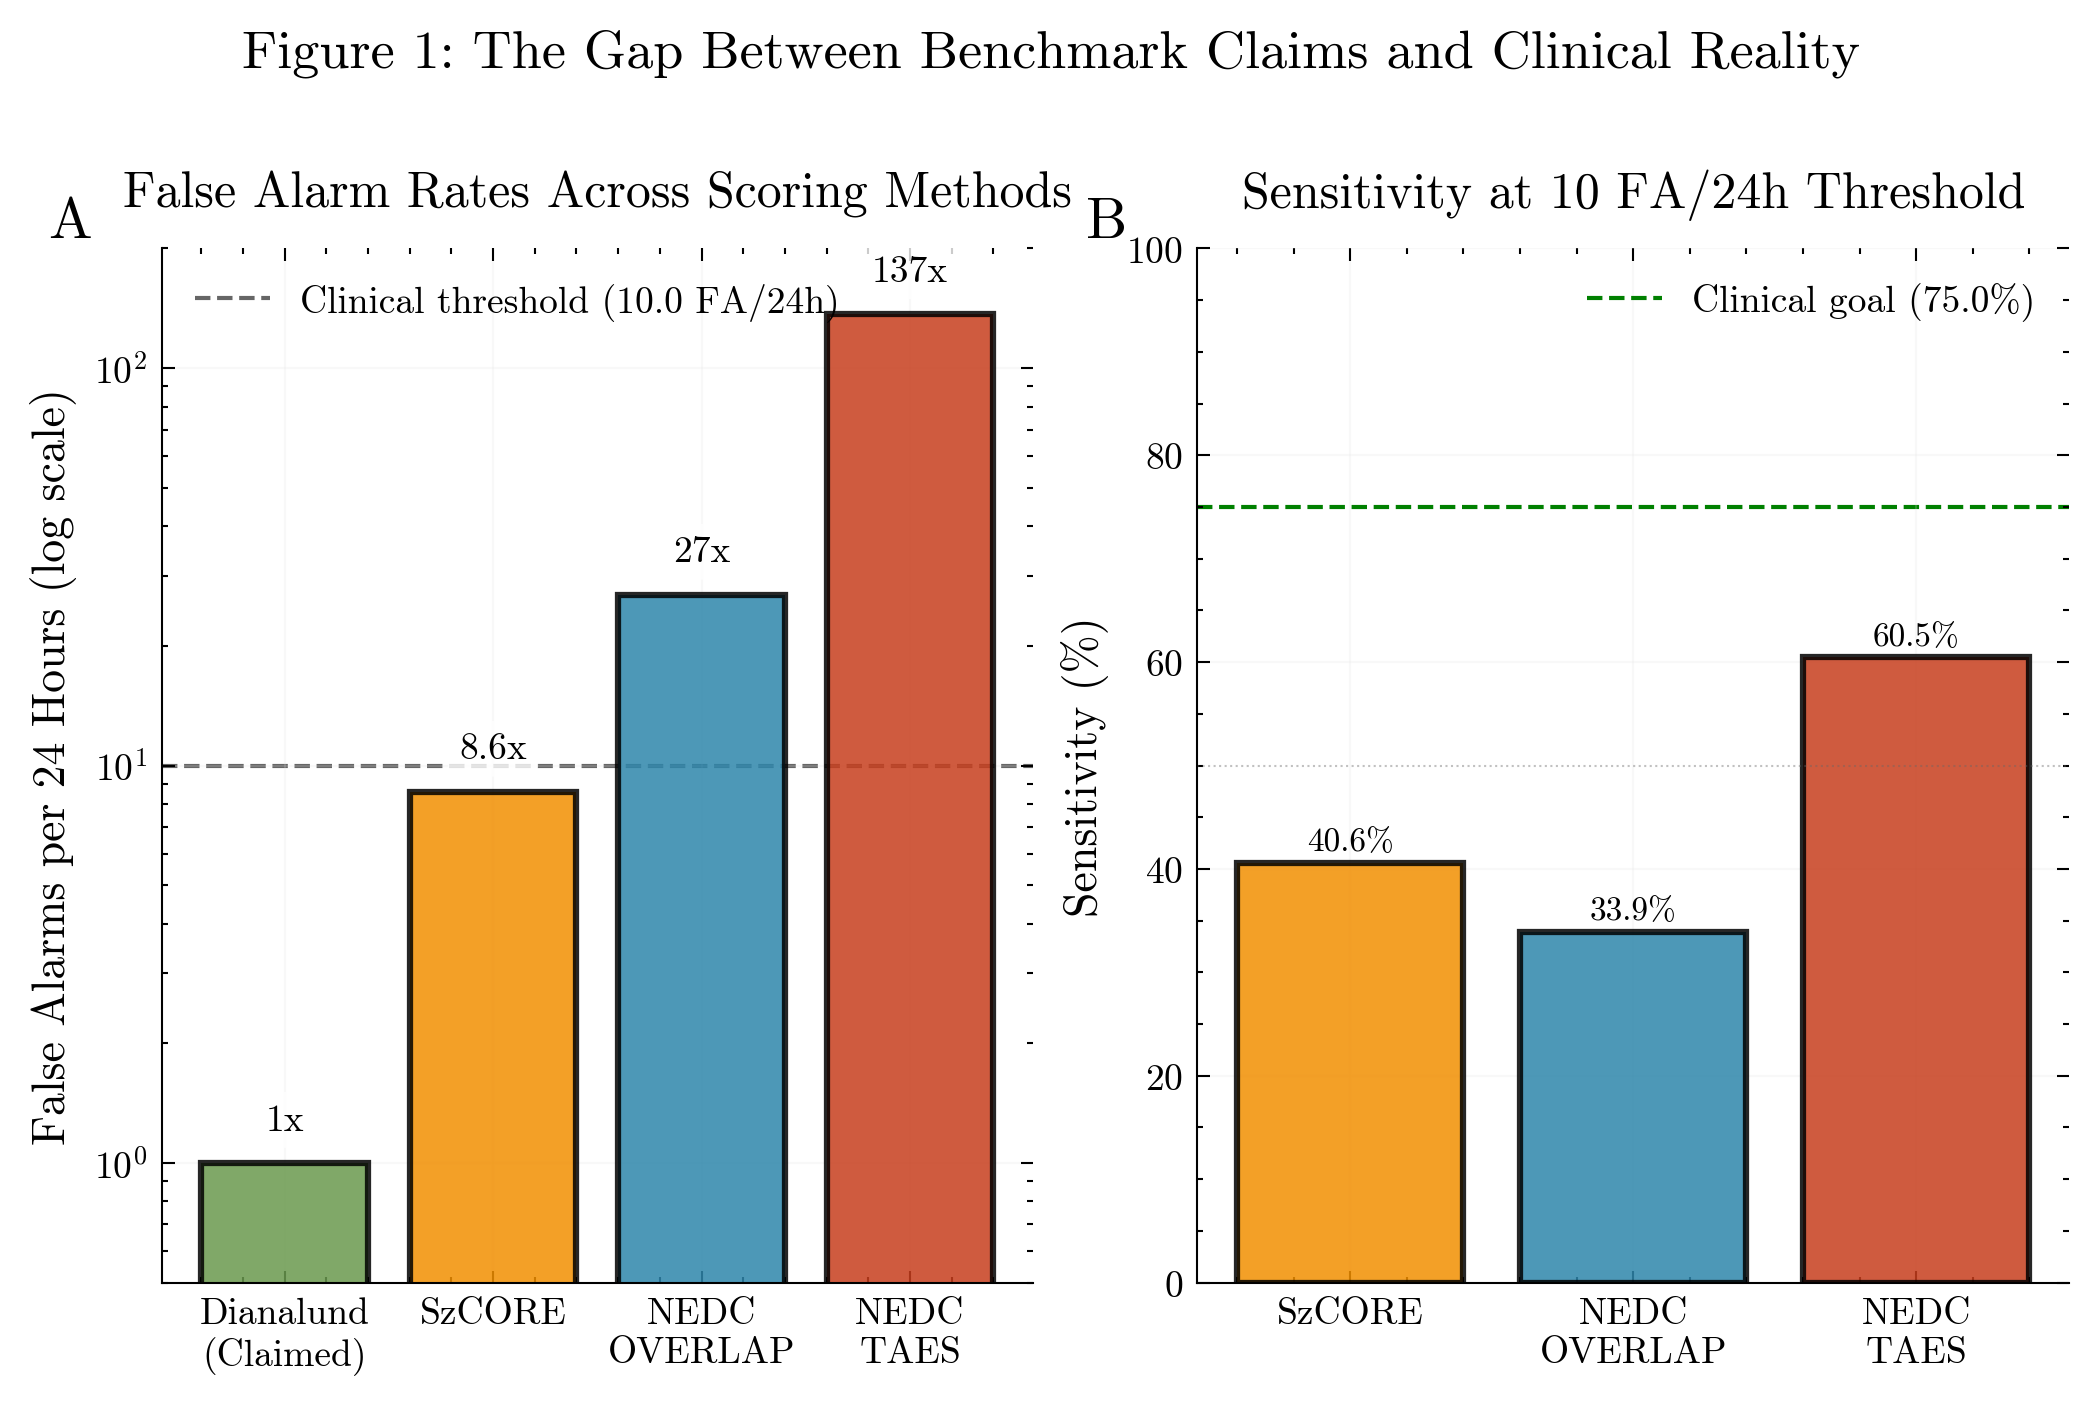
\includegraphics[width=\textwidth]{figures/fig1_performance_gap_optimized.png}
\caption{Performance gap visualization showing the 27--137$\times$ difference between claimed and measured false alarm rates. Panel A shows false alarm rates on a logarithmic scale, comparing Dianalund's claimed performance (1 FA/24h) against our TUSZ evaluation using different scoring methods. Panel B displays sensitivity at the 10 FA/24h operating point across scoring methodologies.}
\label{fig:performance-gap}
\end{figure}

Our contributions extend beyond revealing performance gaps. We provide: (1) a reproducible NEDC v6.0.0 evaluation pipeline for TUSZ, bridging the research-to-clinic evaluation gap; (2) comprehensive operating points for clinical deployment, including evaluation at a clinically-motivated threshold of $\leq$10 FA/24h; (3) quantitative evidence that scoring methodology alone can account for multi-fold performance differences, highlighting the critical need for transparent reporting; and (4) open-source infrastructure enabling the community to replicate and extend our evaluation framework. When optimizing for the 10 FA/24h threshold, SeizureTransformer achieves only 33.90\% sensitivity with NEDC OVERLAP, falling far short of the 75\% sensitivity goal for clinical systems (Roy et al., 2021).

The remainder of this paper is organized as follows. Section 2 provides background and related work on TUSZ, NEDC, and scoring methodologies. Section 3 details our evaluation methodology, including data preparation, model inference, and multi-scorer validation. Section 4 presents comprehensive results across multiple operating points and scoring methods. Section 5 discusses implications for clinical deployment, the need for standardized evaluation, and limitations of current benchmarking practices. Section 6 concludes. Section 7 outlines reproducibility resources and exact rerun procedures.

\end{document}